\chapter[Aplicando Minería de Datos con RapidMiner]{Aplicando Minería de Datos con RapidMiner}
\label{ch:desmin}

\section{Identificación de datos y variables}
\subsection{Recolección de Datos}

Los datos a utilizar en los modelos a presentar en este capítulo son extraídos de la base de datos de la institución privada. Estos datos corresponde a información concreta y confidencial de los años 2014 y 2015 de alumnos de las distintas carreras de ingeniería que imparte la institución. Además se extrae información a través del SIES sobre la institución y sus diferentes carreras de ingeniería con respecto a acreditación e indices de empleabilidad.\\

Los datos proporcionados por la institución se encuentra en un archivo Excel y la información del SIES se encuentra en un sitio web, por lo que se creo una base de datos llamada \textit{Area Staging} conformada por una tabla con toda la información recopilada.\\ 

\subsection{Variables}

Las variables consideradas en este estudio, corresponden al análisis de los constructos del capítulo anterior, además se consideran variables analizadas en el capítulo dos sobre la deserción en Chile.\\

Las variables obtenidas se dividen en tres principales grupos, la primera llamada ``Individual y Educación Media'', corresponde a datos del individuo como su edad y genero, e información previa al ingreso de una institución de educación superior. La segunda llamada ``Institución y Carrera'', corresponde a datos puntuales de la institución y carrera. La tercera llamada ``Alumno'', corresponde a datos sobre actividades, beneficios y rendimiento del alumno.\\



\begin{longtable}{|l|l|l|}
			\hline
			Variable & Tipo & Descripción \\
			\hline \hline
			\endfirsthead
			
			\hline
            Variable & Tipo & Descripción \\
            \hline \hline
            \endhead
			
			\multicolumn{3}{c}{Individual y Educación Media} \\ \hline
			Distancia hogar-institución &  & \\ \hline
			Genero &  & M=2; F=1\\ \hline
			Edad &  & \\ \hline
			Tipo establecimiento de origen &  & \\ \hline
			Notas enseñanza media & & \\ \hline
			Promedio PSU lenguaje y matemáticas &  & \\ \hline
			Prioridad de postulación a carrera & & \\ \hline
			Reingresante & & \\ \hline
			Trabajador & & \\ \hline 
			\multicolumn{3}{c}{Institución y Carrera} \\ \hline
			Tipo Institución &  & \\ \hline
			Acreditación Institucional &  & \\ \hline
			Jornada &  & \\ \hline
			Arancel anual & & \\ \hline
			Empleabilidad al 1er año & & \\ \hline
			Ingreso promedio 4to año & & \\ \hline
			Carrera acreditada & & \\ \hline 
			\multicolumn{3}{c}{Alumno} \\ \hline
			Semestres cursados & & \\ \hline
			Taller profesional realizados & & \\ \hline
			Ha realizado intercambio & & \\ \hline
			Taller certificación realizados & & \\ \hline
			Taller deportivo o cultural & & \\ \hline
			Tiene beca deportiva & & \\ \hline
			Tiene beca de estudio &  & \\ \hline
			Tiene beca de alimento & & \\ \hline
			Tiene crédito &  & \\ \hline
			Promedio notas acumuladas &  & \\ \hline
			Causales acumuladas & & \\ \hline
			Ranking del alumno & & \\ \hline
			Prácticas realizadas & & \\ \hline
			Ha realizado voluntariado social & & \\ \hline
		\caption{Tablou de variables.}
		\label{tabla:Tablou de variables}
\end{longtable}	

Las variables a considerar crean el tablou representado en la Tabla \ref{tabla:Tablou de variables}, estas variables conforman una nueva base de datos, la cual es alimentada por los datos de la base de \textit{Area Staging} creada anteriormente, alguno de estos datos son transformados para generar las variables.\\

Se aclara que algunas variables de este tablou, no podrán ser llenadas con datos previamente recopilados, por lo que para este estudio son considerados con valores nulos para no entorpecer la influencia de otras variables. Sin embargo se recomienda a la institución generar acciones para recopilar estos datos.\\   



\subsection{Modelamiento}

La construcción de los modelos se implementará con la herramienta \textit{RapidMiner} utilizando como entrada el tablou generado anteriormente.\\

La herramienta \textit{RapidMiner} permite a través de operadores, construir un proceso. Los procesos son una serie de pasos constituidos por operadores.\\

\begin{figure}[H]
	\centering 
	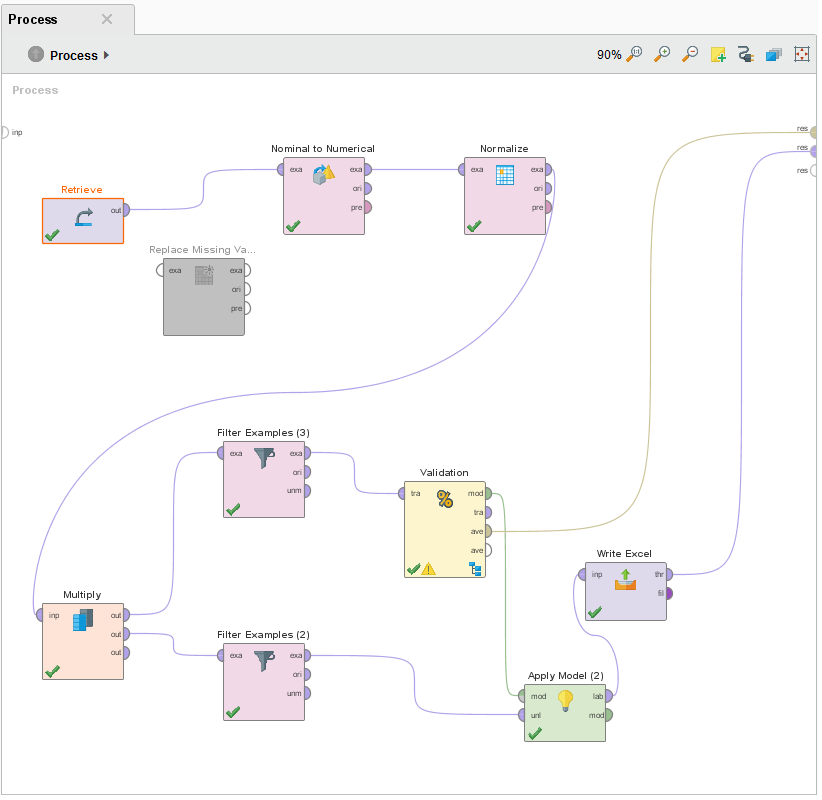
\includegraphics[width=12cm,height=7cm] {proceso.png} 
	\caption[Proceso de Predicción]{Proceso de Predicción}
	\label{fig:proceso}
\end{figure}

\begin{figure}[H]
	\centering 
	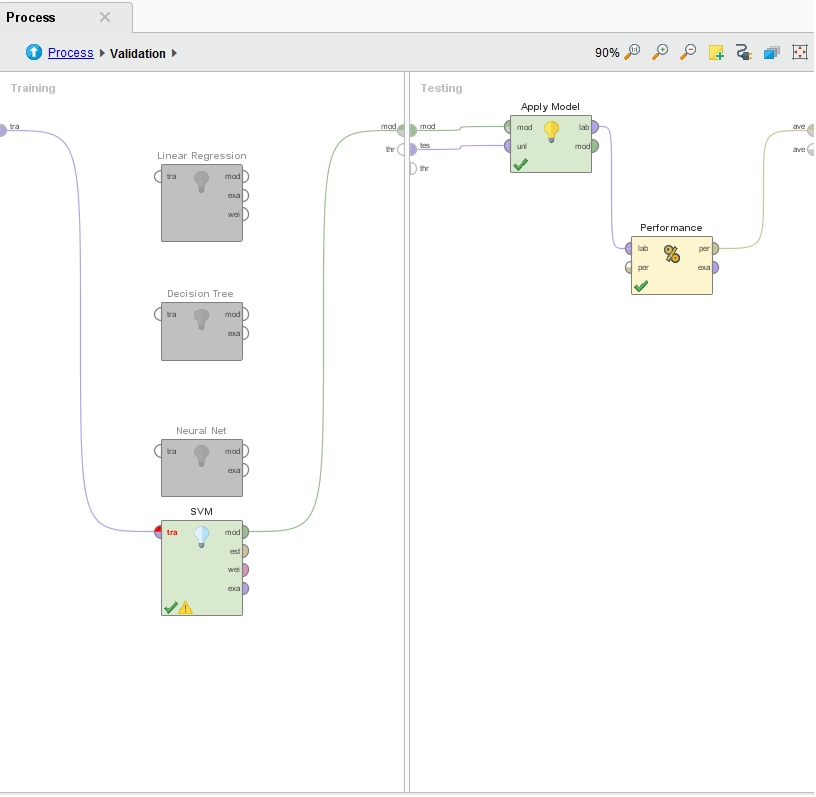
\includegraphics[width=12cm,height=7cm] {provalidacion.png} 
	\caption[Validación]{Validación}
	\label{fig:validacion}
\end{figure}